

The success of a mixed finite element formulation crucially depends on a proper choice of the local interpolations of the velocity and the pressure. 

%----------------------------------------------------------------------
\subsubsection{The compatibility condition (or LBB condition)}






\subsubsection{The bi/tri-linear velocity - constant pressure element ($Q_1\times P_0$)}

\includegraphics[width=3cm]{images/under_construction}

%----------------------------------------------------------------------
\subsubsection{The bi/tri-quadratic velocity - discontinuous linear pressure element ($Q_2 \times P_{-1}$)}

\includegraphics[width=3cm]{images/under_construction}

%----------------------------------------------------------------------
\subsubsection{The bi/tri-quadratic velocity - bi/tri-linear pressure element ($Q_2 \times Q_1$)}

\includegraphics[width=3cm]{images/under_construction}


This element, implemented in penalised form, is discussed in \cite{been79} and the follow-up paper \cite{been80}. CHECK

Biquadratic velocities, bilinear pressure. See Hood and Taylor. The element satisfies the inf-sup condition \cite{hugh}p215. 

\begin{center}
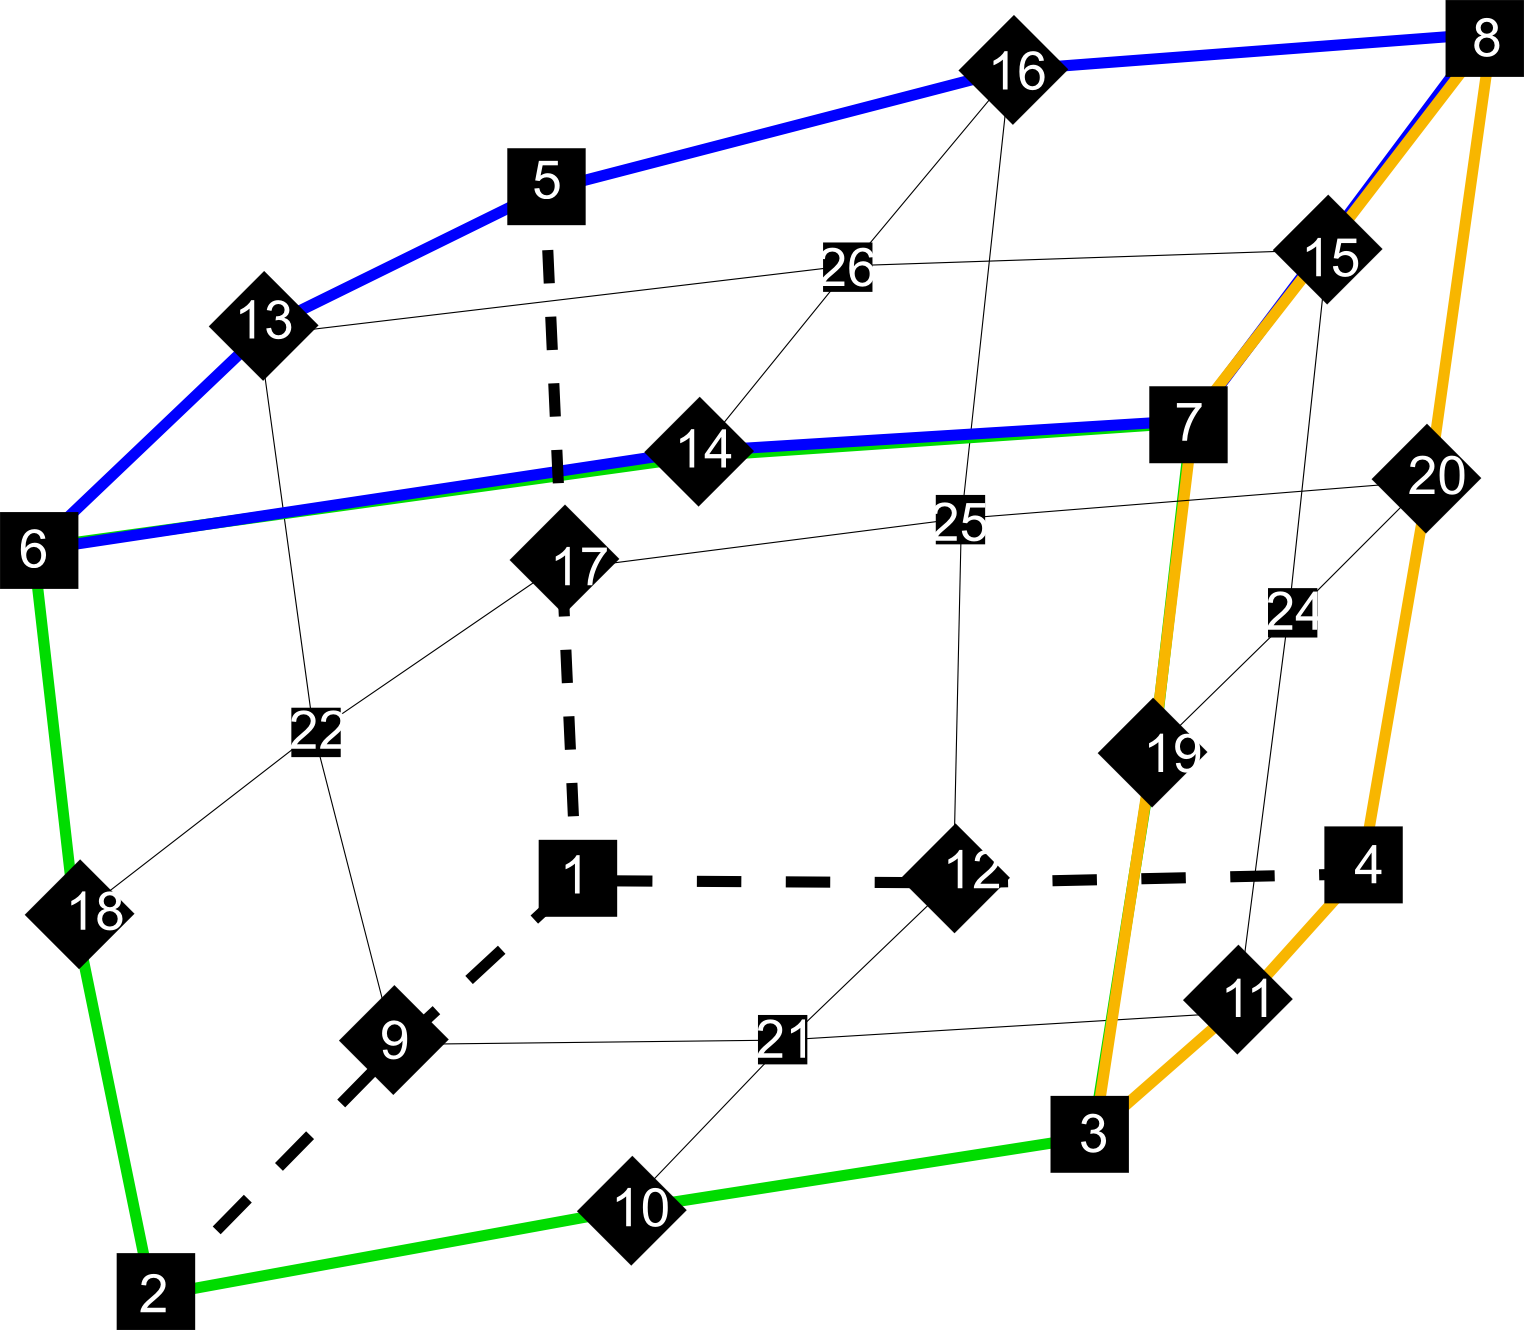
\includegraphics[width=6cm]{images/q2q1/q2numering}
\end{center}


%----------------------------------------------------------------------
\subsubsection{The stabilised bi/tri-linear velocity -  bi/tri-linear pressure element ($Q_1\times Q_1$-stab)}

\includegraphics[width=3cm]{images/under_construction}

%----------------------------------------------------------------------
\subsubsection{The MINI triangular element ($P_1^+\times P_1$)}

\includegraphics[width=3cm]{images/under_construction}

%----------------------------------------------------------------------
\subsubsection{The quadratic velocity - linear pressure triangle ($P_2\times P_1$)}

\includegraphics[width=3cm]{images/under_construction}

From \cite{segal}.
Taylor-Hood elements (Taylor and Hood 1973) 
are characterized by the fact that the pressure is continuous in the region $\Omega$. 
A typical example is the quadratic triangle (P2P1 element).
In this element the velocity is approximated by a quadratic polynomial and the pressure by a
linear polynomial. One can easily verify that both approximations are continuous over 
the element boundaries. 
It can be shown, Segal (1979), that this element is admissible if at least 3 elements 
are used. The quadrilateral counterpart of this triangle is the $Q_2\times Q_1$ element.




%----------------------------------------------------------------------
\subsubsection{The Crouzeix-Raviart triangle ($P_2^+\times P_{-1}$)}

\includegraphics[width=3cm]{images/under_construction}

From \cite{daks08}: seven-node Crouzeix-Raviart triangle with quadratic velocity shape functions enhanced by a cubic bubble function and discontinuous linear interpolation for the pressure field [e.g., Cuvelier et al., 1986]. This element is stable and no additional stabilization techniques are required [Elman et al., 2005].

From \cite{segal}. These elements are characterized by a discontinuous pressure; 
discontinuous on element boundaries. 
For output purposes (printing, plotting etc.) these discontinuous pressures are averaged 
in vertices for all the adjoining elements.

The most simple Crouzeix-Raviart element is the non-conforming linear triangle 
with constant pressure ($P_1\times P_0$).

p248 of Elman book. satisfies LBB condition. 

%----------------------------
\subsection{Other elements}

P1P0

P1P1

Q2Q2

P2P2

